\documentclass[border=8pt]{standalone}
\usepackage[T1]{fontenc}
\usepackage{helvet}
\renewcommand{\familydefault}{\sfdefault}
\usepackage{amsmath}
\usepackage{tikz}
\usetikzlibrary{positioning, arrows.meta}

% colours
\definecolor{bias}{RGB}{190,60,50}
\definecolor{conditioned}{RGB}{232,232,242}

\begin{document}
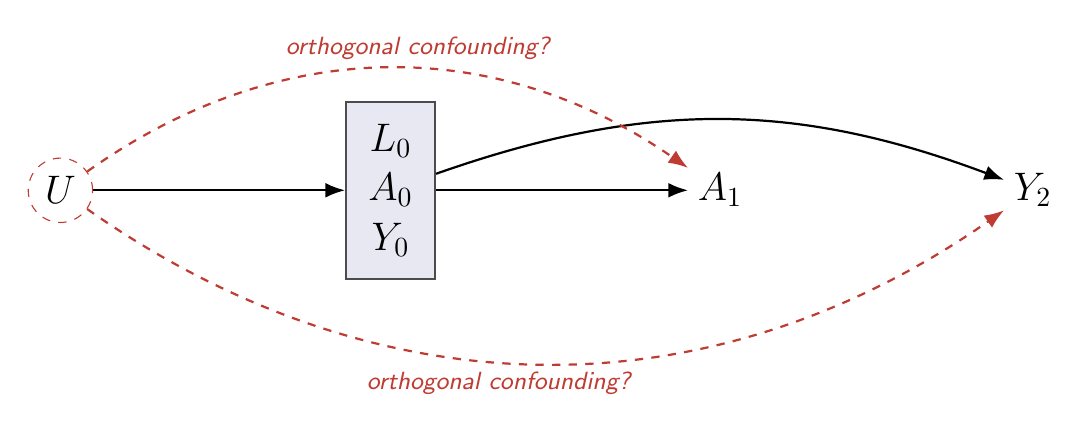
\begin{tikzpicture}[
    node distance=3.2cm,
    every node/.style={font=\Large},
    arrow/.style={-{Latex[length=2.5mm]}, thick},
    biasarrow/.style={arrow, dashed, color=bias},
]

% nodes (time flows left to right)
\node[draw=bias, dashed, circle, inner sep=3pt] (U) {$U$};
\node[rectangle, draw=black!70, thick, fill=conditioned,
      align=center, right=of U, inner sep=8pt] (L) {$L_0$\\$A_0$\\$Y_0$};
\node[right=of L] (A) {$A_1$};
\node[right=of A] (Y) {$Y_2$};

% structural arrows (blocked by conditioning on baseline)
\draw[arrow] (U) -- (L);
\draw[arrow] (L) -- (A);
\draw[arrow, bend left=20] (L) to (Y);

% potential residual confounding (orthogonal to measured baseline history)
\draw[biasarrow, bend left=35] (U) to
    node[pos=0.55, above, font=\small\itshape, text=bias]
    {orthogonal confounding?} (A);
\draw[biasarrow, bend right=35] (U) to
    node[pos=0.45, below, font=\small\itshape, text=bias]
    {orthogonal confounding?} (Y);

\end{tikzpicture}
\end{document}
